%%%%%%%%%%%%%%%%%%%%%%%%%%%%%%%%%%%%%%%%%
% Beamer Presentation
% LaTeX Template
% Version 1.0 (10/11/12)
%
% This template has been downloaded from:
% http://www.LaTeXTemplates.com
%
% License:
% CC BY-NC-SA 3.0 (http://creativecommons.org/licenses/by-nc-sa/3.0/)
%
%%%%%%%%%%%%%%%%%%%%%%%%%%%%%%%%%%%%%%%%%

%----------------------------------------------------------------------------------------
%	PACKAGES AND THEMES
%----------------------------------------------------------------------------------------

\documentclass{beamer}

\mode<presentation> {

% The Beamer class comes with a number of default slide themes
% which change the colors and layouts of slides. Below this is a list
% of all the themes, uncomment each in turn to see what they look like.

%\usetheme{default}
%\usetheme{AnnArbor}
%\usetheme{Antibes}
%\usetheme{Bergen}
%\usetheme{Berkeley}
%\usetheme{Berlin}
%\usetheme{Boadilla}
%\usetheme{CambridgeUS}
%\usetheme{Copenhagen}
%\usetheme{Darmstadt}
%\usetheme{Dresden}
%\usetheme{Frankfurt}
%\usetheme{Goettingen}
%\usetheme{Hannover}
%\usetheme{Ilmenau}
%\usetheme{JuanLesPins}
%\usetheme{Luebeck}
\usetheme{Madrid}
%\usetheme{Malmoe}
%\usetheme{Marburg}
%\usetheme{Montpellier}
%\usetheme{PaloAlto}
%\usetheme{Pittsburgh}
%\usetheme{Rochester}
%\usetheme{Singapore}
%\usetheme{Szeged}
%\usetheme{Warsaw}

% As well as themes, the Beamer class has a number of color themes
% for any slide theme. Uncomment each of these in turn to see how it
% changes the colors of your current slide theme.

%\usecolortheme{albatross}
%\usecolortheme{beaver}
%\usecolortheme{beetle}
%\usecolortheme{crane}
%\usecolortheme{dolphin}
%\usecolortheme{dove}
%\usecolortheme{fly}
%\usecolortheme{lily}
%\usecolortheme{orchid}
%\usecolortheme{rose}
%\usecolortheme{seagull}
%\usecolortheme{seahorse}
%\usecolortheme{whale}
%\usecolortheme{wolverine}

%\setbeamertemplate{footline} % To remove the footer line in all slides uncomment this line
%\setbeamertemplate{footline}[page number] % To replace the footer line in all slides with a simple slide count uncomment this line

%\setbeamertemplate{navigation symbols}{} % To remove the navigation symbols from the bottom of all slides uncomment this line
}

\usepackage{graphicx} % Allows including images
\usepackage{booktabs} % Allows the use of \toprule, \midrule and \bottomrule in tables
\usepackage{listings}
\usepackage{amsmath}
\usepackage{algpseudocode,algorithm,algorithmicx}


%----------------------------------------------------------------------------------------
%	TITLE PAGE
%----------------------------------------------------------------------------------------

\title[Binary Trees/Binary Search Trees]{Binary Trees/Binary Search Trees} % The short title appears at the bottom of every slide, the full title is only on the title page

\author{Jonathan Windle} % Your name
\institute[UEA] % Your institution as it will appear on the bottom of every slide, may be shorthand to save space
{
University of East Anglia \\ % Your institution for the title page
\medskip
\textit{J.Windle@uea.ac.uk} % Your email address
}
\date{\today} % Date, can be changed to a custom date

\begin{document}

\begin{frame}
\titlepage % Print the title page as the first slide
\end{frame}

\begin{frame}[allowframebreaks]
\frametitle{Overview} % Table of contents slide, comment this block out to remove it
\tableofcontents % Throughout your presentation, if you choose to use \section{} and \subsection{} commands, these will automatically be printed on this slide as an overview of your presentation
\end{frame}

%-----------------------------------------------------------------
\section{Binary Trees}
\subsection{Intro}
\begin{frame}
\frametitle{Intro}
\begin{itemize}
\item Tree structures are {\color{green}Non-Linear}.
\item A {\color{red} Binary Tree} $T$, on a set of elements $E$ is either:
\begin{itemize}
\item empty, or
\item consists of a finite collection of nodes, each containing an element of $E$, and which contains a particular node called the {\color{purple} root} of $T$, with the remaining nodes of $T$ partitioned into to binary tress, called {\color{orange} left sub-tree} and {\color{magenta} right sub-tree} respectively.
\end{itemize}
\end{itemize}
\end{frame}
%-----------------------------------------------------------------
\subsection{Terminology}
\begin{frame}
\frametitle{Terminology}
\begin{itemize}
\item {\color{blue} nodes/vertices} - contain elements of $T$.
\item {\color{blue} parent} - Every node except for the root has a unique parent node.
\item {\color{blue} child} - if $p$ is the parent of $c$ thee $c$ is a child of $p$.
\item {\color{blue} siblings} - two nodes are siblings if they have the same parent node.
\item {\color{blue} ancestor} - Node $a$ is an ancestor of node $d$ if either $a$ is the parent of $d$ or $a$ is the parent of an ancestor of $d$.
\item {\color{blue} descendant} - Node $d$ is a descendant of $a$ if $a$ is an ancestor of $d$.
\item {\color{blue} leaf} - a node with no child.
\item {\color{blue} external} - another name for a leaf node.
{\color{blue} internal} - a non-leaf node, i.e. a nde with  at least one child.
\item {\color{blue} level} - if $n$ is the root node, then $level(n) = 0$, otherwise $level(n) = level(parent(n))+1$.
\item {\color{blue} height} - $height(T)=max_{n \in T}level(n)$ (Height $T$ is also called the level of the tree).
\end{itemize}
\end{frame}
%----------------------------------------------------------------
\subsection{Traversing a Tree}
\begin{frame}
\frametitle{Traversing a Tree}
\begin{columns}[c]
\column{.45\textwidth}
\begin{itemize}
\item {\color{red} Preorder:}
\begin{itemize}
\item Visit root
\item Visit left sub-tree in preorder
\item Visit right sub-tree in preorder
\end{itemize}
\item {\color{green} Inorder:}
\begin{itemize}
\item Visit left sub-tree inorder
\item Visit root
\item Visit righ sub-tree inorder.
\end{itemize}
\item {\color{purple} Postorder:}
\begin{itemize}
\item Visit left sub-tree in postorder.
\item Visit right sub-tree in postorder.
\item Visit root.
\end{itemize}
\end{itemize}
\column{.45\textwidth}
\vline
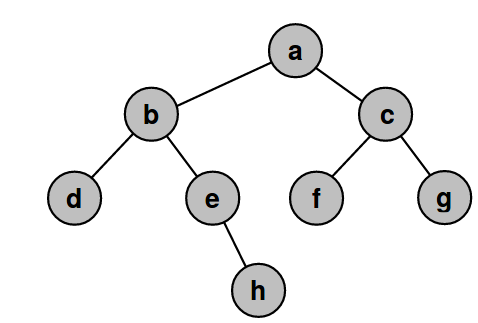
\includegraphics[width = .8\textwidth]{bTree.png}
\begin{itemize}
\item {\color{red} a,b,d,e,h,c,f,g}
\item {\color{green} d,b,e,h,a,f,c,g}
\item {\color{purple} d,h,e,b,f,g,c,a}
\end{itemize}
\end{columns}
\end{frame}
%-----------------------------------------------------------------
\section{Binary Search Trees}
\subsection{Intro}
\begin{frame}
\frametitle{Intro}
\begin{itemize}
\item A Binary Search Tree, $t$, is a binary tree, either it is empty or each node in the tree has an associated identifier, or {\color{red} key} from a totally ordered set of keys, such that:
\begin{itemize}
\item The keys of all nodes in the left sub-tree of $t$ are less than the key of the root of $t$
\item The keys of all nodes in the right sub-tree of $t$ are greater than the key of the root $t$.
\item The left and right sub-trees of t are themselves binary search trees.
\end{itemize}
\end{itemize}
\end{frame}
%----------------------------------------------------------------
\subsection{Insertion}
\begin{frame}
\frametitle{Insertion}
\begin{enumerate}
\item Search for the given key:
\begin{itemize}
\item Use two reference variables, $t$ and $p$.
\item $t$ references the current \texttt{TreeNode}
\item $p$ references the parent node of $t$.
\end{itemize}
\item If the given key is found, do nothing.
\item Otherwise, $p$ references the \texttt{TreeNode} which will be the parent of the incoming node:
\begin{itemize}
\item update p.left or p.right as appropriate.
\end{itemize}
\end{enumerate}
\end{frame}
%-----------------------------------------------------------------
\subsection{Deletion}
\begin{frame}
\begin{enumerate}
\item Locate node $t$ if present nd the parent node $p$ like in insertion.
\item If found, three cases need to be considered:
\begin{enumerate}
\item Node contains no children:
\begin{itemize}
\item Just set the left or right reference field in $p$ as appropriate to null.
\end{itemize}
\item Node has a single child:
\begin{itemize}
\item Set the left or right reference field in $p$ to reference \texttt{t.left} or \texttt{t.right} as appropriate.
\end{itemize}
\item Node to be deleted has two children:
\begin{itemize}
\item The {\color{red} inorder} successor of $t$ must take its place.
\item The inorder successor cannot have a left child, right child can be moved up to take  its place.
\item See example on next page:
\end{itemize}
\end{enumerate}
\end{enumerate}
\end{frame}
\begin{frame}
\frametitle{Deletion Example}
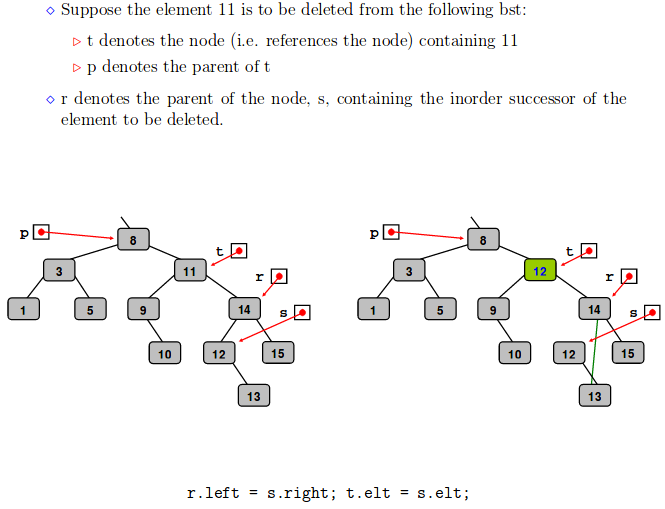
\includegraphics[scale=0.5]{deletion.png}
\end{frame}

%------------------------------------------------------------------
\subsection{Balanced Binary Search Trees}
\begin{frame}
\frametitle{Balanced Binary Search Trees}
\begin{itemize}
\item Given a BST is balanced, then searching a BST is $O(logn)$.
\item A BST, $t$ is {\color{red} height-balanced} if either:
\begin{itemize}
\item $t = 0$
\item $t \neq 0$ and:
\begin{itemize}
\item $left(t)$ and $right(t)$ are height balanced or,
\item $| height(left(t)) - height(right(t))| \leq 1$.
\end{itemize}
\end{itemize}
\item AVL trees are height-balanced BST.
\item $balance(t) = height(left(t)) - height(right(t))$
\end{itemize}
\end{frame}
%-----------------------------------------------------------------
\subsubsection{Balance example}
\begin{frame}
\frametitle{Balance example}
\begin{itemize}
\item Dashed lines represent where insertions can take place.
\item B = Balanced insertion.
\item U = Unbalanced insertion.
\end{itemize}
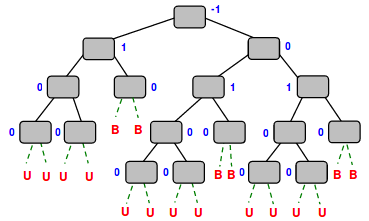
\includegraphics[scale=0.5]{balanced.png}
\end{frame}
%-----------------------------------------------------------------
\subsubsection{Case +1 node becomes unbalanced}
\begin{frame}
\frametitle{Case +1 node becomes unbalanced}
\begin{itemize}
\item The balance of a node, $a$ is +1.
\item Suppose $a$ is the youngest ancestor to become unbalanced when a new node is inserted into the bst.
\begin{itemize}
\item $balance(a) = 1 \implies left(a) \neq 0$.
\end{itemize}
\item Let $b$ be the left child of $a$.
\item Deduce that $balance(b) = 0$.
\begin{itemize}
\item $balance(b) = 0 \implies height(left(b)) = height(right(b)) = n$
\item $(height(b) = n+1) \land (balance(a)=1) \implies height(right(a)) = n$
\end{itemize}
\end{itemize}
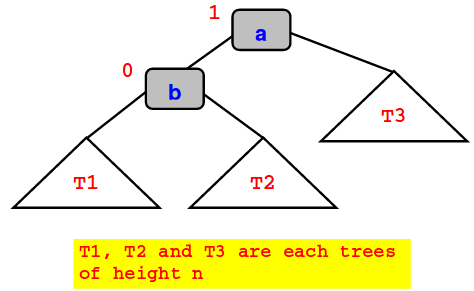
\includegraphics[scale=0.25]{balance.png}
\end{frame}
%-----------------------------------------------------------------
\subsubsection{Transform unbalanced to balanced}
\begin{frame}
\frametitle{Transform unbalanced to balanced}
\begin{itemize}
\item Right rotation:
\end{itemize}
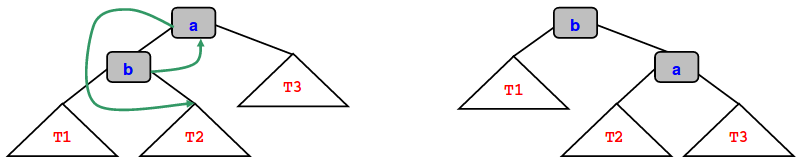
\includegraphics[scale=0.25]{right.png}
\begin{itemize}
\item Left rotation:
\end{itemize}
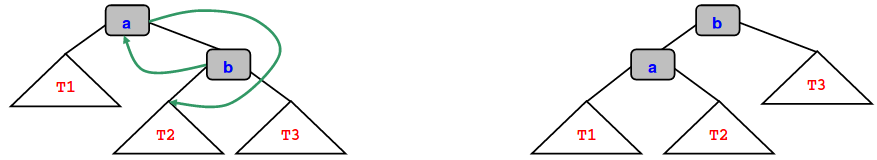
\includegraphics[scale=0.25]{left.png}
\begin{itemize}
\item Any previously balances BST made unbalanced by a single insertion can be re-balanced by performing either a single rotation or a double rotation using the above.
\end{itemize}
\end{frame}
%-----------------------------------------------------------------
\begin{frame} 
\Huge{\centerline{The End}}
\end{frame}

\end{document}